\section{System-Level Framework}
\label{sec:system}

This section describes the overall framework and operation of our
prediction-based controller.

\subsection{Programmer Annotation}

% Programmer annotation
\begin{figure}
  \begin{center}
    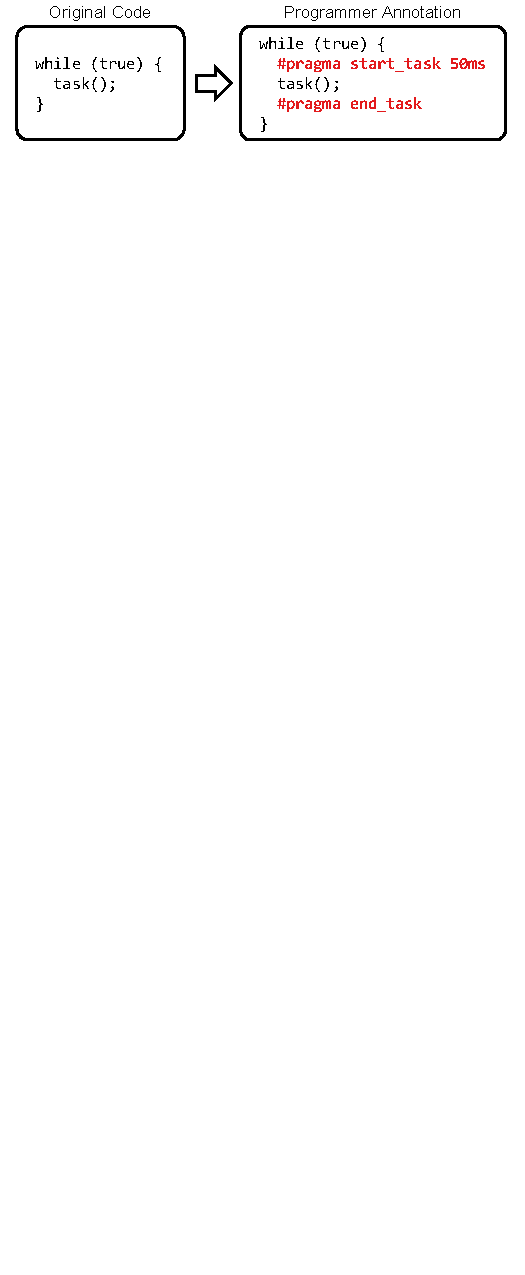
\includegraphics{exec_time_prediction/figs/programmer_annotation.pdf}
    \caption{Example of programmer annotation to mark task boundaries and time budgets.}
    \label{fig:system.programmer_annotation}
  \end{center}
\end{figure}

In order to identify tasks and their time budgets, programmer annotation is
required. The programmer must annotate the start and the end of a task and the
desired response-time requirement.
Figure~\ref{fig:system.programmer_annotation} shows an example of this
annotation.  For ease of analysis and to ensure that tasks that start always
end, we require the start and end of a task to be within one function.
Arbitrary code paths can be modified to fit this model by using a wrapper
function or re-writing the code. Multiple non-overlapping tasks can be
supported, though we only considered one task in the applications we tested.

\subsection{Off-line Analysis}

% High-level flow of framework
\begin{figure*}
  \begin{center}
    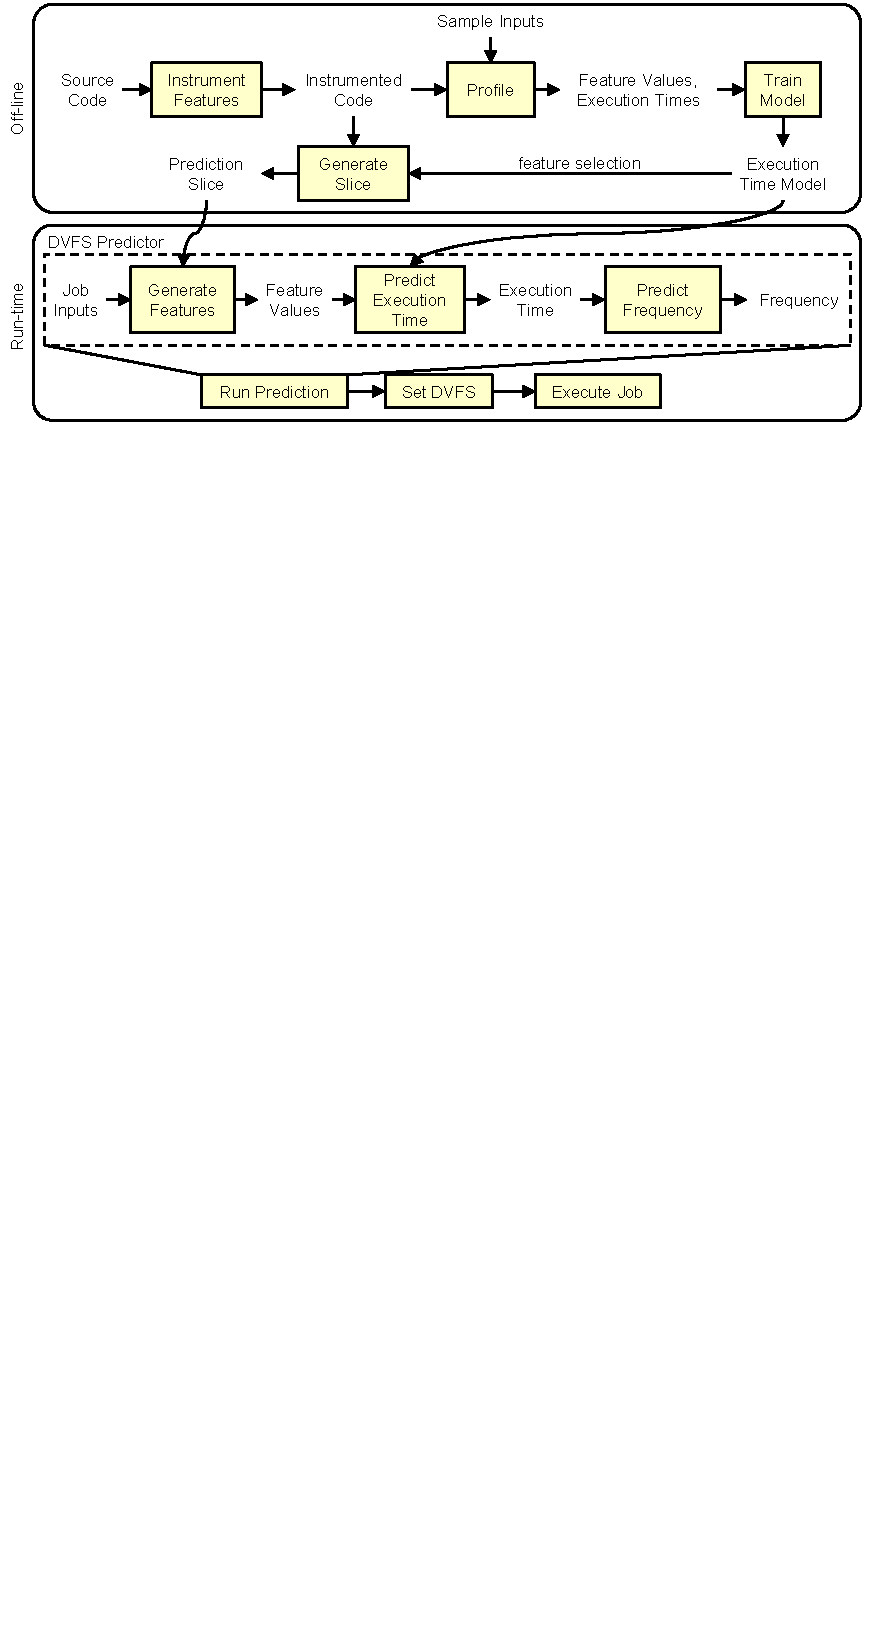
\includegraphics{exec_time_prediction/figs/high_level_flow.pdf}
    \caption{Overall flow for prediction-based DVFS control.}
    \label{fig:system.high_level_flow}
  \end{center}
\end{figure*}

Figure~\ref{fig:system.high_level_flow} shows the overall flow of our framework
for creating prediction-based DVFS controllers. Given programmer annotation to
identify tasks, we can automatically instrument these tasks to record control flow
features. Off-line, we profile these tasks in order to collect
traces of feature values and job execution times.
This is used to train our execution time prediction model, as
described in Section~\ref{sec:prediction.model}. Since execution time depends
on the specific hardware and platform that an application is run on, profiling
and model training needs to be done for the platform that the application will
be run on. For common platforms, the program developer can perform this
profiling and distribute the trained model coefficients with the program.
Alternatively, profiling can be done by the user during the application's
installation.

The trained execution time model only requires a subset of all the features to
perform prediction. Thus, this information is used to eliminate code for
calculating unneeded features. 
Program slicing is then used to create a minimal code fragment to calculate
the needed control flow features. 
Note that since the
features needed depends on the training of the execution time prediction model,
which is platform-dependent, the features needed could vary across platforms.
However, we expect the features that are needed are primarily a function of the
task semantics (i.e., execution time variations across control paths) rather
than the platform it is run on. In fact, we compared the predictions made for
an x86-based (Intel Core i7) platform when using the features selected for an
ARM-based ODROID-XU3 platform and for the features selected for the x86
platform itself. For all but three of the benchmarks we tested, the features
selected were exactly the same.  For one of these, the features selected by the
x86 platform were a subset of those selected by the ARM platform and so the
predicted times were exactly the same. For the remaining two benchmarks, the
predicted times differed by less
than 3\%. Although we had to re-train the execution time model coefficients,
the same prediction slice was applicable across both platforms.

\subsection{Run-time Prediction}

% Slice operation choices
\begin{figure}
  \begin{center}
    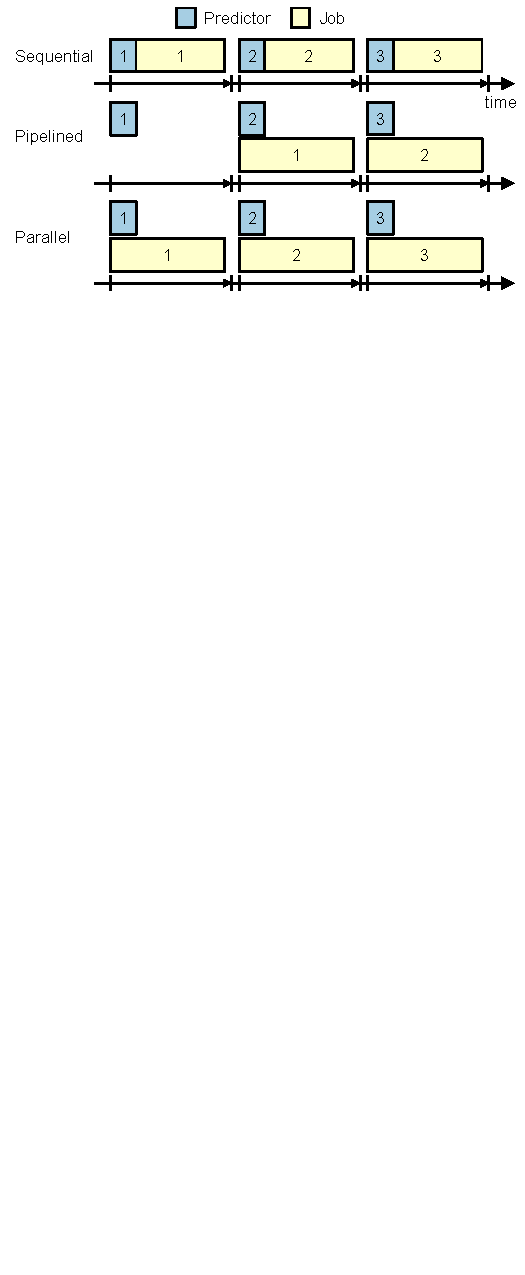
\includegraphics{exec_time_prediction/figs/predictor_operation.pdf}
    \caption{Options for how to run predictor.}
    \label{fig:prototype.predictor_operation}
  \end{center}
\end{figure}

The prediction slice, execution time predictor, and frequency predictor are
combined to form the \emph{DVFS predictor} or simply \emph{predictor}
There are several options for how to run the predictor in relation to jobs.
Figure~\ref{fig:prototype.predictor_operation} shows some of these options. 
The simplest approach is to run the slice just before the execution of
a job. This uses up part of the time budget to perform slicing, as mentioned
in Section~\ref{sec:prediction.dvfs}. However, if this time is low, then the
impact is minimal.

% Although this means that part of the job's deadline time is used for
% prediction, if the prediction time is small, then the impact should be
% minimal. In addition, one problem with running sequentially is that the slice
% could have side effects (e.g., write to global variables) which could cause
% errors in the job execution.

An alternative option would be to run the predictors and jobs in a parallel,
pipelined manner such that during job $i$, the predictor for job
$i+1$ is run. This ensures that the DVFS decision is ready at the start of a job with
no impact on time budget from the predictor.
However, this assumes that information needed by the prediction slice, 
specifically the job inputs and program state, 
is ready one job in advance. This is not possible for interactive
tasks which depend on real-time user inputs or tasks which are not
periodic.

The predictor could also be run in parallel with the task. This avoids
the issue of needing input values early.  In terms of time budget, this mode of
operation still reduces the effective budget by the predictor execution time.
However, part of the task also executes during the prediction time. By
accounting for this, the energy savings may be higher than running in a
sequential manner.  Running in parallel also avoids the issue of side-effects
caused by the prediction slice that was discussed in
Section~\ref{sec:prediction.features}. However, running in parallel either
requires forking off the predictor for each job or sharing data with a
dedicated predictor thread, both of which can introduce overhead.

For our target applications, we found that the execution time of the predictor
was low. Thus, we decided to run the predictor and task in a sequential
manner. For applications which require more complicated predictors, these
alternative operation modes may be beneficial.
